\section{Результаты (1)}\label{section:bidirected}

В данном главе будет рассмотрена модификация алгоритма~\ref{algo:PI}, основанная на ослаблении условия на граф, а именно, на ``предположении'', что он является неориентированным. Также будет доказана корректность данной модификации для двунаправленных графов и языка Дика, а также для неориентированных графов и некоторых видов грамматик.

Для неориентированных графов отношение достижимости равно отношению ``принадлежать одной компоненте связности''. Поддерживать добавление рёбер и проверку связности в неориентированном графе можно с помощью структуры данных Система Непересекающихся Множеств. 

% Система Непересекающихся Множеств (СНМ)
\begin{definition}
  \textit{Система Непересекающихся Множеств (или СНМ)}\footnote{Disjoint-set/union–find data data structure}~\cite{Galler1964}~--- структура данных для работы с непересекающимися множествами. Её интерфейс включает следующие операции:
  \vspace{-\topsep}
  \begin{itemize}
    \setlength\itemsep{-0.1em}
    \item \textit{MakeSet}$(x)$~--- создаёт новое множество, состоящее из одного элемента $x$
    \item \textit{Find}$(x)$~--- возвращает элемент-представитель множества, содержащего $x$. Для всех элементов одного множества элемент-представитель одинаков
    \item \textit{Union}$(x, y)$~--- объединяет множества, содержащие элементы $x$ и $y$
  \end{itemize}
\end{definition}

\subsection{Алгоритм, основанный на неориентированном транзитивном замыкании}

В листинге~\ref{algo:NP} приведён псевдокод алгоритма.

\begin{algorithm}[h]
  \floatname{algorithm}{Listing}
  \begin{algorithmic}[1]
  \caption{Алгоритм достижимости для РКА, основанный на неориентированном ИТЗ}
  \label{algo:NP}
  \Function{UndirectedRSMReachability}{$\cool{R}$}
      \State{$A \gets$ Empty adjacency matrix}
      \State{$Q \gets$ Empty Queue}
      \State{$D \gets$ DSU($|\bigcup\limits_{i=1}^k Q_i|$)}
      \For{$i \in 1..k$}
          \For{$u \xrightarrow{c} v \in \delta_i$}
              \State{$Q.Push(\q{u, v, i})$}
          \EndFor
      \EndFor
      \While{$Q$ is not Empty}
          \State{$\q{u, v, i} \gets Q.Pop()$}
          \If{$u \in En_i \wedge v \in En_i$}
              \Comment{Нашли новый путь}
              \State{$A \gets A \cup getEdges(i, u, v)$}
              \State{$Q.PushAll(getEdges(i, u, v))$}
              \State{$D.Union(u, v)$}
              \Comment{Добавляем новые рёбра}
          \EndIf
      \EndWhile
  \State \Return $A$
  \EndFunction
  \end{algorithmic}
\end{algorithm}

Для реализации используются две вспомогательные структуры данных: очередь $Q$, хранящая рёбра, которые были добавлены в граф, но ещё не обработаны (как и в оригинальном алгоритме), и СНМ $D$, поддерживающая компоненты связности и поиск новых путей $\langle$стартовое состояние$\to$конечное состояние$\rangle$. 

Опишем подробно структуру используемой СНМ (в листинге~\ref{algo:DSU} приведён псевдокод).

\algblockdefx[Structure]{Structure}{EndStructure}
[1]{{\bf Structure} #1}
{}

\begin{algorithm}[h]
  \floatname{algorithm}{Listing}
  \begin{algorithmic}[1]
  \caption{Система Непересекающихся Множеств}
  \label{algo:DSU}
  \Structure{DisjointSets}
      \Function{DisjointSets}{$V$}
          \For{$v \in V$}
              \State{$P[v] \gets v$}
              \Comment{Предкок}
              \State{$R[v] \gets 0$}
              \Comment{Ранг}
          \EndFor
          \For{$v \in En(V)$}
              \State{$En[v] \gets \{v \}$}
              \Comment{Список стартовых вершин поддерева}
          \EndFor
          \For{$v \in Ex(V)$}
              \State{$Ex[v] \gets \{v \}$}
              \Comment{Список конечных вершин поддерева}
          \EndFor
      \EndFunction
      \Function{Find}{$v$}
          \If{$P[v] = v$}
              \Return $v$
          \EndIf
          \Return $P[v] = Find(P[v])$
          \Comment{Эвристика сжатие путей}
      \EndFunction
      \Function{Union}{$u, v$}
          \State{$u \gets Find(u)$}
          \State{$v \gets Find(v)$}
          \If{$u = v$}
              \Return
          \EndIf
          \If{$R[u] > R[v]$}
              \State{$Swap(u, v)$}
              \Comment{Ранговая эвристика}
          \EndIf
          \State{$Q.PushAll(\{ \q{en_u, ex_v}~|~en_u \in En[u], ex_v \in Ex[v] \})$}
          \State{$Q.PushAll(\{ \q{en_v, ex_u}~|~en_v \in En[v], ex_u \in Ex[u] \})$}
          \Comment{Добавление новых рёбер}
          \State{$En[v] \gets En[v] \cup En[u]$}
          \State{$Ex[v] \gets Ex[v] \cup Ex[u]$}
          \State{$R[v] \gets \max(R[v], R[u]+1)$}
          \State{$P[u] = v$}
          \Comment{Объединение компонент}
      \EndFunction
  \EndStructure
  \end{algorithmic}
\end{algorithm}

За основу взята стандартная реализация \cite{Hopcroft1973} на подвешенных деревьях, использующая обе эвристики: сжатие путей и ранговую. 

% \TODO: \textit{Надо ли её расписывать?}
% Ненадо

Дополнительно в корнях хранятся списки всех начальных и конечных состояний компоненты. При добавлении ребра в операции \textit{Union} перебираются все пары начальная/конечная вершина из двух компонент и соответствующие им рёбра добавляются в рабочую очередь $Q$. 

\TODO: (подумоть) можно ли добавлять сразу много рёбер и сжимать их дфсом (как Борувка)?

\subsection*{Время работы}

\begin{theorem}
  На РКА из $|V|$ состояний и $|E^{*}|$ рёбрах в транзитивном замыкании, алгоритм~\ref{algo:NP} отработает за время $\O(|V| + |E^{*}| \alpha(|V|))$
\end{theorem}

\begin{proof}
  Как и в алгоритме~\ref{algo:PI} проход по внешнему циклу и добавление новых рекурсивных рёбер отработает за $\O(|E^{*}|)$, так как каждое ребро транзитивного замыкания рассмотрится не более одного раза.

  Осталось оценить время работы $|E^{*}|$ вызовов функции \textit{Union}. Каждый из них совершает 2 вызова функции \textit{Find}, каждый из которых отработает за амортизированное $\O(\alpha(|V|))$. Также, если вершины находились в разных компонентах, происходит перебор всех пар начальное-конечное состояние. Однако, этот перебор суммарно переберёт каждое ребро транзитивного замыкания не более одного раза, так что суммарно отработает за $\O(|E^{*}|)$.

  Итого, время работы алгоритма составляет $\O(|V| + |E^{*}| \alpha(|V|))$ ($\O(|V|)$ берётся из создания СНМ на $|V|$ множеств). 
\end{proof}

\subsection{Корректность для неориентированных графов и некоторых классов грамматик}

\TODO: может, в мусорку этот subsection?

\subsection{Корректность для двунаправленных графов и языка Дика}

\begin{theorem}\label{th:bidir_corr}
  Алгоритм~\ref{algo:NP} работает корректно на двунаправленных графах и языке Дика.
\end{theorem}

% \textit{Напоминание, что для языка Дика контекстно-свободная достижимость $\to$ Дикова достижимость}

Для доказательства потребуется следующее вспомогательное утверждение:

\begin{lemma}\label{lemma:bidir_equiv}
  Для вершин двунаправленных графов отношении Диковой достижимости является отношением эквивалентности.
  % For bidirected graphs the Dyck-reachability relation forms an equivalence, i.e., for all bidirected graphs $G$, for every pair of nodes $u$, $v$, we have that $v$ is Dyck-reachable from $u$ iff $u$ is Dyck-reachable from $v$.
\end{lemma}
\begin{proof}

  Действительно, если инвертировать (заменить все $(_i$ на $)_i$ и наоборот) и развернуть правильную скобочную последовательность, то получится так же правильная скобочная последовательность.\\
  Пример: ПСП: `\texttt{([]())}' $\to$ развёрнутая: `\texttt{))(][(}' $\to$ инвертированная: `\texttt{(()[])}'.

\end{proof}

\begin{note}
  В доказательстве для простоты будет рассматриваться язык Дика $\cool{D}_2$ (на двух типах скобок). Все рассуждения обобщаются на случай $k$ типов скобок.
\end{note}

\begin{note}    
  Для данного алгоритма будем использовать нестандартный РКА для языка Дика (изображён на рис.~\ref{img:dyck_rsm})

  \begin{figure}[H]
      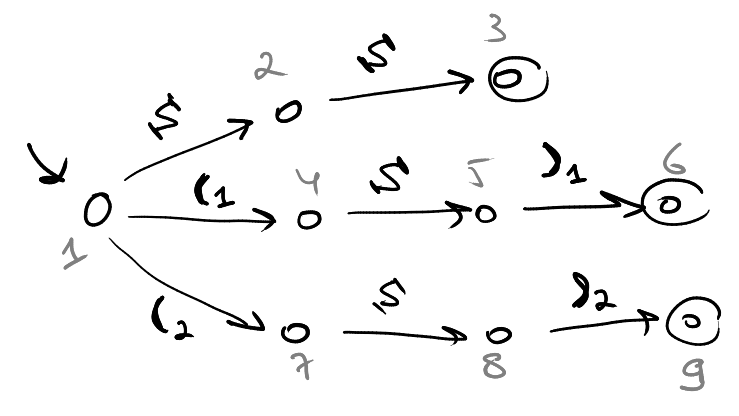
\includegraphics[width=0.75\linewidth]{img/dyck_rsm}
      \caption{РКА для языка Дика $\cool{D}_2$.\\ Заметим, что он содержит всего одну компоненту.}
      \label{img:dyck_rsm}
  \end{figure}

  \TODO: нарисовать красиво (+ eps переход)

\end{note}

\begin{proof}{Теоремы~\ref{th:bidir_corr}}

  Достаточно доказать, что для любой пары состояний $e \in En_i, ex \in Ex_i$ существование неориентированного пути эквивалентно существованию ориентированного.

  $\Leftarrow$ (ориентированный $\SO$ неориентированный)

  Очевидно, если есть ориентированный путь $en \path ex$, то если убрать ориентацию этот путь всё ещё останется корректным.

  $\Rightarrow$ (неориентированный $\SO$ ориентированный)

  Для начала заметим, что компонента нашего РКА (произведения РКА языка Дика и входного графа) образует слоистую структуру: на $i$-ом слое~--- состояния $\q{q_i, u}$, где $q_i$~--- $i$-ое состояние РКА языка Дика. Т.к. РКА Дика топологически отсортирован, все рёбра ведут из слоя с меньшим номером в слой с большим.

  % At first, note that the Kronecker product $G \otimes \mathcal{G}$ forms some kind of a layered structure~--- $i$-th layer consists of vertices $(q_i, v)$, where $q_i$ is $i$-th RSM state. Because RSM is topologically sorted ({\color{red}{TODO}}), every edge $(q_i, u) \rightarrow (q_j, v)$ goes forward.

  Назовём неориентированный путь \textit{простым}, если он проходит по каждому слою не боле одного раза.

  Пусть есть неориентированный путь $p \colon en \path ex$. Покажем, что тогда существует \textit{простой} путь $p' \colon en \path ex$. Заметим, что так как рёбра идут только из слоя с меньшим номером в слой с большим, то простой путь из первого слоя в последний на самом деле направлен согласно исходной ориентации рёбер. Т.е. такой простой путь и будет искомым.

  Доказывать это утверждение (про наличие простого пути $p'$) будем индукцией по длине пути.

  % We will call path \textit{simple} if it visits every layer no more than once.

  % We prove the claim by induction on the $l$ (path length).

  Очевидно, утверждение верно для путей длины 1, 2 и 3~--- все они и так являются простыми.

  Рассмотрим путь $p$ длины $\ge 4$, он уже не будет простым. Найдём первую \textit{точку перегиба} пути~--- вершину, из который путь идёт в состояние на слое с меньшим номером.

  % Clearly the result is true for $l \le 3$, because the only way to achive final vertex in $1, 2$ or $3$ edges is by a simple vertical path (which exists in the original graph too).

  % Otherwise (if $l \ge 4$), path is not simple. 

  % Consider the first flex point of the path, that is the vertex $(q_i, v)$ such that edges $(q_j, u) \rightarrow (q_i, v)$ and $(q_i, v) \rightarrow (q_k, w)$ are in the path and $j, k \le i$ (so, the path is convex at this point).

  Внимательно посмотрев на РКА языка Дика, можно заметить, что все состояния имеют входящую степень 1 (для этого и нужен был нестандартный вид), так что рёбра, соседствующие в пути $p$ с точкой перегиба имеют одинаковую метку и идут на один и тот же уровень. Обозначим эти рёбра как $\q{q_i, u} \to \q{q_j, v} \to \q{q_i, w}$ ($\q{q_j, v}$~--- точка перегиба).

  Рассмотрим все 3 варианта возможной метки на рёбрах вокруг точки перегиба.

  % Looking at the grammar graph we can notice, that every state has indegree $\le 1$. So at the flex point there are actually two same-labeled edges (that is, $j = k$). 

  % There can be three different types of labels on those edges:

  \begin{itemize}
    \item открывающая скобка $(_k$

      $p \colon (q_1, u) \rightarrow (q_{4/7}, v) \rightarrow (q_1, w) \rightarrow \dots \rightarrow (q_f, z)$.

      Рёбра с меткой $(_k$ соответствуют рёбрам входного графа, а именно рёбрам $u \xrightarrow{(_k)} v$ и $w \xrightarrow{(_k)} v$. Заметим, что тогда, по двунаправленности графа, существует и ребро $v \xrightarrow{)_k} w$, дающее вместе с ребром $u \xrightarrow{(_k)} v $ путь $(_k )_k$ из $u$ в $w$, порождающий $S$-ребро $\q{q_1, u} \to \q{q_2, w}$. Также, по предположению индукции существует простой путь $\q{q_1, w} \to \q{q_f, z}$, а значит есть и $S$-ребро $\q{q_2, w} \to \q{q_3, z}$. Вместе эти два ребра формируют просто путь $\q{q_1, u} \to \q{q_2, w} \to \q{q_3, z}$, что и хотелось.

    \item $S$-метки

      $p \colon (q_1, a) \rightarrow \dots \rightarrow (q_i, u) \rightarrow (q_j, v) \rightarrow (q_i, w) \rightarrow \dots \rightarrow (q_f, z)$.

      По лемме~\ref{lemma:bidir_equiv}, из наличия дикового пути $w \path v$ следует наличие дикового пути $v \path w$. Вместе два диковых пути $u \path v$ и $v \path w$ образуют один путь $u \path w$. 

      Сожмём этот путь в одну вершину $uw$. Получим более короткий путь, для него по предположению индукции существует аналогичный простой путь. Если этот простой путь не проходит через вершину $uw$, то он и является ответом. Иначе. Если вершина $uw$ находится на 2, 4 или 7 слое, то следующее за ней ребро в простом пути имеет метку $S$, а значит, вместе с диковым путём $u \path w$ собирается в один диков путь (по правилу $S \to SS$, как в случае $(_k$). Если же $uw$ находится на 1 слое, то весь путь от неё до $z$~--- один диков путь, который так же складывается с путём $u \path w$.  

      % $\mathcal{G}$ contains $S$-labeled edges $u \xrightarrow{S} v$ and $w \xrightarrow{S} v$. Since $\mathcal{G}$ is bidirected, then by \ref{r1} $v \xrightarrow{S} u$ and $v \xrightarrow{S} w$. Combining $u \xrightarrow{S} v$ and $v \xrightarrow{S} w$ we get that $u \xrightarrow{S} w$. 

      % No we want to sort of contract this edge, joining $u$ and $w$ (on the $j$-th level). Then we can get (by induction hypothesis) the directed path from $(q_0, a) \rightsquigarrow (q_f, z)$. If new path does not contain joined $uw$ vertex, then that's the answer. Otherwise we can split this vertex back, inserting between $u$ and $w$ the $S$-labeled path (that one, from $u \xrightarrow{S} w$ edge). We can do it, because the both of these paths form correctly matched parenthesis ({\color{red}{TODO}}: we can prove this using stack-based checking algorithm).

      % \textit{Two other cases can be proved the same way, but I find it a little dishonest}

    \item закрывающая скобка $)_k$

      $p \colon (q_1, a) \rightarrow \dots \rightarrow (q_i, u) \rightarrow (q_f, v) \rightarrow (q_i, w) \rightarrow \dots \rightarrow (q_f', z)$.

      % Since $\alpha_l$-labeled edges could only be added on the initialization stage, 
      % graph $\mathcal{G}$ contains edges $u \xrightarrow{\overline{\alpha_l}} v$ and $w \xrightarrow{\overline{\alpha_l}} v$. Notice, that cause $\mathcal{G}$ is bidirected, it also has to contain edges $v \xrightarrow{\alpha_l} u$ and $v \xrightarrow{\alpha_l} w$.

      По предположению индукции, существует простой путь $a \path v$, так что есть $S$-ребро $\q{q_1, a} \to \q{q_2, v}$. Поймём, почему будет и ребро $\q{q_2, v} \to \q{q_3, z}$, которое вместе с предыдущем даёт искомый простой путь.

      По двунаправленности графа, из наличия ребра $w \xrightarrow{)_k} v$ следует наличие ребра $v \xrightarrow{(_k)} w$. Вместе с изначальным $\eps$-ребром $w \xrightarrow{S} w$ и остатком пути $\q{q_i, w} \path \q{q_f', z}$ получаем более короткий путь, для которого, по предположению индукции существует аналогичный простой путь. Он и порождает второе ребро $\q{q_2, w} \to \q{q_3, z}$. 

      % By induction, we get that $a \xrightarrow{S} v$. Now we will construct a second part of the path: $(q_0, v) \xrightarrow{\alpha_l} (q_{j-1}, w) \xrightarrow{S} (q_j, w) \rightsquigarrow (q_f, z)$ ($q_{j-1}, w) \xrightarrow{S} (q_j, w)$ ~--- initial $S$-loop). By induction, we have directed simple version of this path, so $v \xrightarrow{S} z$. 

      % Combining this two paths ($a \xrightarrow{S} v$ and $v \xrightarrow{S} z$) we get $a \xrightarrow{SS} z \Rightarrow a \xrightarrow{S} z$~--- desired path.

    \begin{figure}[H]
        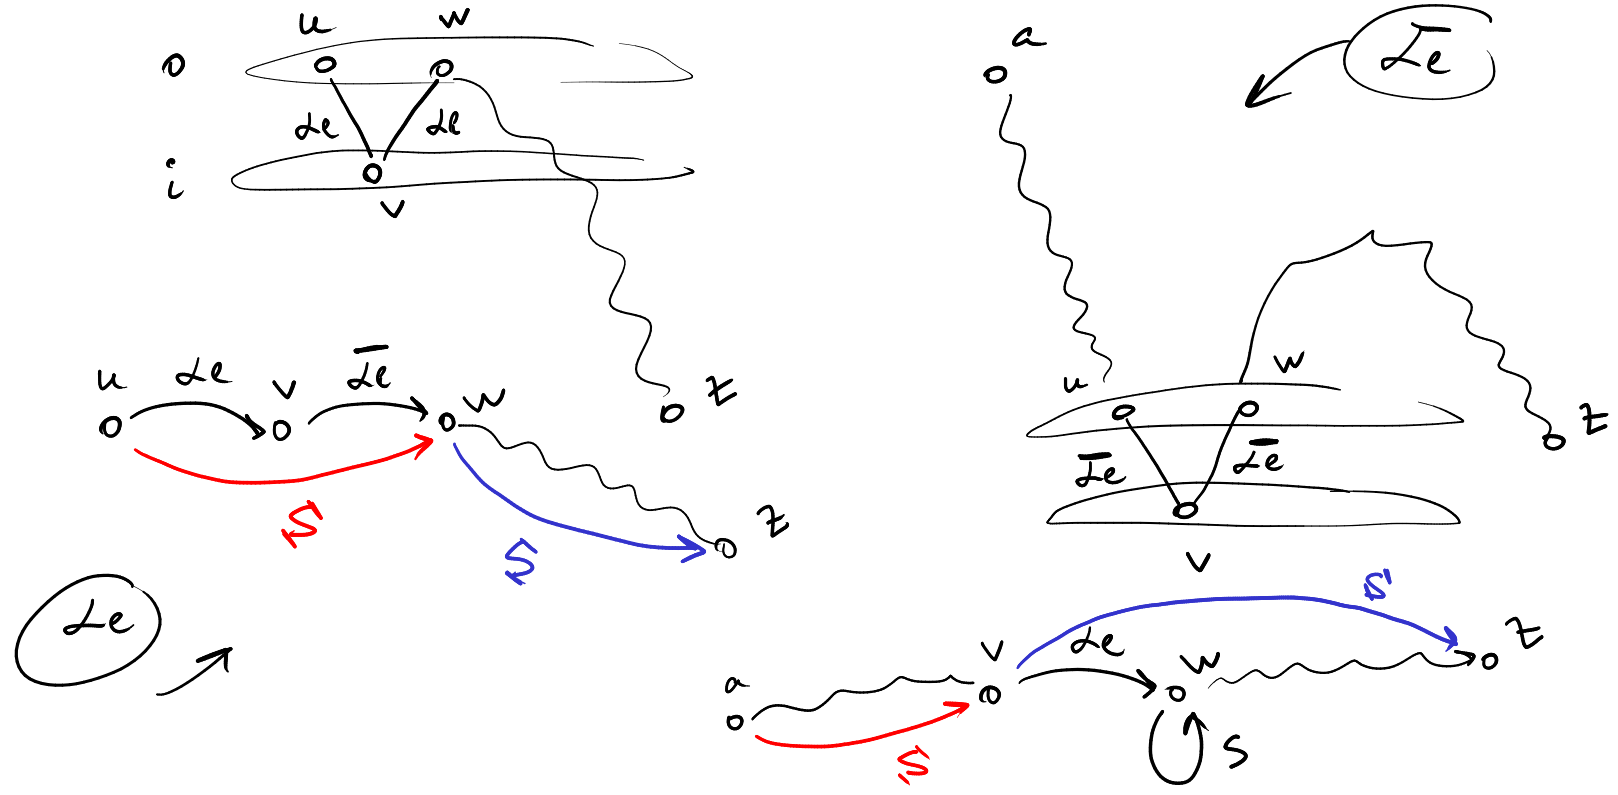
\includegraphics[width=\linewidth]{img/th_proof_img}
    \end{figure}

    \TODO: норм картинка
  \end{itemize}

\end{proof}

\subsection{Выводы и результаты по главе}


\includegraphics[width=0.75\linewidth]{img/hole}

\TODO